\documentclass{article} % For LaTeX2e
\usepackage{nips13submit_e,times}
\usepackage{hyperref}
\usepackage{url}
\usepackage{tikz,amsmath}
\usepackage[procnames]{listings}
%\documentstyle[nips13submit_09,times,art10]{article} % For LaTeX 2.09


\title{Project Report: Digit Recognizer}

\author{
Jimmy Lin (xl5224) \\
Department of Computer Science\\
University of Texas at Austin\\
Austin, TX 78712 \\
\texttt{JimmyLin@utexas.edu} \\
%{{{ For More Author
\And
Jisong Yang (jy7226) \\
Department of Statistical Scientfic Computation\\
University of Texas at Austin\\
Austin, TX 78712 \\
\texttt{jsyang993@gmail.com} \\
%\AND
%Coauthor \\
%Affiliation \\
%Address \\
%\texttt{email} \\
%\And
%Coauthor \\
%Affiliation \\
%Address \\
%\texttt{email} \\
%\And
%Coauthor \\
%Affiliation \\
%Address \\
%\texttt{email} \\
%(if needed)\\
%}}}
}

% The \author macro works with any number of authors. There are two commands
% used to separate the names and addresses of multiple authors: \And and \AND.
%
% Using \And between authors leaves it to \LaTeX{} to determine where to break
% the lines. Using \AND forces a linebreak at that point. So, if \LaTeX{}
% puts 3 of 4 authors names on the first line, and the last on the second
% line, try using \AND instead of \And before the third author name.

\newcommand{\fix}{\marginpar{FIX}}
\newcommand{\new}{\marginpar{NEW}}

\nipsfinalcopy % Uncomment for camera-ready version


% TODO: Find a report guideline 
% TODO: 
\begin{document}


\maketitle

\begin{abstract}
    BACKGROUND. The idea of recognizing digit . 
    The topic of this project is trying to figure out a model that is good at
    determing the human-understood digit within an handwritten image of a
    single digit. Kaggle competition. 
    We attempted the simplest deformation model called IDM and figure out the
    computational solution throught distributed and concurrent system.

\end{abstract}

\section{Introduction}
\subsection{Problem Description}
% MOTIVATION SENTENCE
Recognizing hand-written characters has long been a hot topic in artificial
intelligence community. 
% KEY CONCEPT (PROBLEM) ILLUMINATION
Handwriting recognition is the ability of a computer to receive and
interpret intelligible handwritten input from sources such as paper documents,
photographs, touch-screens and other devices.
% SUMMARIZE THE SOLUTION
In the past decades, many probabilistic or non-probabilistic algorithms have
been exploited to effectively solve this problem, including K-nearest
neighbour, random forest, and well-known neural network. 


 \subsection{Motivations} \label{Motivation}
% APPLICATION OF THIS PROBLEM 
As to the historical application of handwriting recognition, 
it can be traced back to early 1980s.  There are plenty of commercial products
incorporating handwriting recognition as a replacement for keyboard input were
introduced. The hardware application continued to develop
in the following decades.  Until the recent years, Tablet PCs can be regarded
as a special notebook computer that is outfitted with a digitizer tablet and a
stylus, and allows a user to handwrite text on the unit's screen. In addition,
highly efficient handwriting recognizers were developed in real world to apply
on the zip codes detection.

\begin{figure}[h]
    \centering
    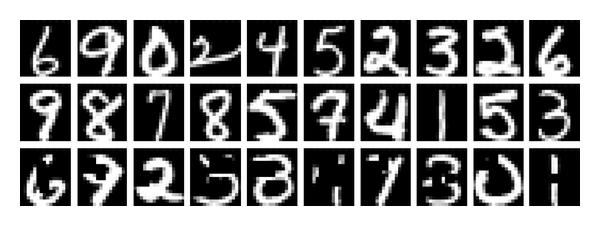
\includegraphics[width=3.5in,height=1.5in]{./857453.jpg}\\
    \caption{Digit Recognition Examples}
\end{figure}

% RELATED WORKS/SOLUTION
Plenty of mature solutions has already been developed to existence in solving
the handwriting problem. 
Since 2009, the recurrent neural networks and deep feedforward neural networks
developed in the research group of Jürgen Schmidhuber at the Swiss AI Lab
IDSIA have outshined many other models in competitions.
% POSSIBLE IMPROVEMENTS?
The fact that existing algorithms are powerful in recognizing digits does not
remove possibility of further improvement. The chance of improvement lies in
reduction of computational complexity for recognizing digits in higher degree.

\subsection{Dataset}
As mentioned previously, the dataset provided by the holder of digit
recognition kaggle competition came from the famous MNIST dataset.
The {\bf MNIST database (Mixed National Institute of Standards and Technology
    database)} is a large database of handwritten digits that is commonly used for
training various image processing systems. It was created by "re-mixing" the
samples from NIST's original datasets. The creators felt that since NIST's
training dataset was taken from American Census Bureau employees, while the
testing dataset was taken from American high school students, NIST's complete
dataset was too hard. Furthermore, the black and white images from NIST were
normalized to fit into a 20x20 pixel bounding box and anti-aliased, which
introduced grayscale levels.

The competition holder provides us two csv data files, train.csv and test.csv.
The data files train.csv and test.csv contain gray-scale images of hand-drawn
digits, from zero through nine.  Each image is 28 pixels in height and 28
pixels in width, for a total of 784 pixels in total. Each pixel has a single
pixel-value associated with it, indicating the lightness or darkness of that
pixel, with higher numbers meaning darker. This pixel-value is an integer
between 0 and 255, inclusive.

The training data set (in train.csv), has 42,000 rows and 785 columns. The first column, called
"label", is the digit that was drawn by the user. The rest of the columns
contain the pixel-values of the associated image.  Each pixel column in the
training set has a name like pixelx, where $x$ is an integer between 0 and
783, inclusive. To locate this pixel on the image, suppose that we have
decomposed $x$ as $x = i \times 28 + j$, where $i$ and $j$ are integers
between 0 and 27, inclusive. Then pixelx is located on row $i$ and column $j$
of a $28 \times 28$ matrix (indexing by zero).  
\begin{align}
\begin{matrix}
000 & 001 & 002 & 003 & \dots & 026 & 027 \\
028 & 029 & 030 & 031 & \dots & 054 & 055 \\
056 & 057 & 058 & 059 & \dots & 082 & 083 \\
\vdots  & \vdots & \vdots    & \vdots   & \dots & \vdots  & \vdots  \\
728 & 729 & 730 & 731 & \dots & 754 & 755 \\
756 & 757 & 758 & 759 & \dots & 782 & 783 
\end{matrix}
\end{align}

The test data set (in test.csv), is the same as the training set, except that it
does not contain the "label" column and the test data has 28,000 images in total.

\subsection{Report Organization}
% ORGANIZATION OF THIS REPORT
In this report, we will illuminate the motivation of digit recognition
problem on section \ref{Motivation}. In section \ref{Details}, the
 main models exploited in this project will be sequentially present to
 reader. Those algorithms are PCA-KNN, Neural Network, Multi-class SVM and
 Deformation Model. For each model, the algorithmic description, the
 motivation of attempting that algorithm and finally relevant issues on
 practical implementation will be indicated. 

\section{Implementation Details} \label{Details}
\subsection{PCA-KNN} 
% INTRODUCITON OF PCA
{\bf Principal Component Analysis} (PCA) is a statistical procedure that uses
orthogonal transformation to convert a set of observations of possibly
correlated variables into a set of values of linearly uncorrelated variables
called principal components. Typically, the number of principal components is
no more than the number of original variables. That is to say, a particular
subspace, whose bases are independent to each other, is generated by such
tranformation. This transformation is defined in such a way that the first
principal component has the largest possible variance, and each succeeding
component in turn has the highest variance possible under the constraint that
it is orthogonal to the preceding components. In section \ref{Comparison}, the
performance comparisons of different algorithms will be illustrated and after
which, we will make conclusion about which one achieve the best performance. 

\begin{figure}[h]
    \centering
    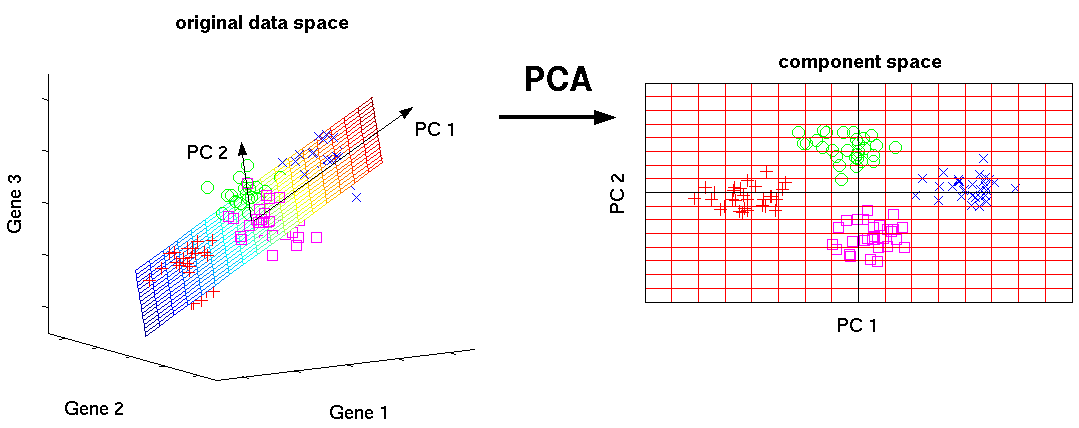
\includegraphics[height=2.6in,width=5.2in]{./images/PCA.png}
    \caption{Principle Component Analysis}
\end{figure}

% WHY USE PCA
In our project, we make use of PCA as dimensionality reduction for preprocessing the raw input image data.
Since the raw data explictly characterize the gray value of each pixels, each
handwritten instance is extremely high-dimensional ($28\times 28 = 784$ in
total). Although directly using the raw input data avoids loss of information,
the computational complexity would be unresonably large. Put it another way,
we have to think of a way to compromise the ultimate accuracy to achieve a
less computational cost on that algorithm. 

\newcommand{\knn}{$k$-Nearest Neighour }
% PROBLEM OF PCA
However, several details matter significantly to the effect of PCA. One is the number
of principal components employed. If too many principal components are used,
it is far from reaching the goal of dimensionality reduction. However, we may
lose useful information for latter prediction if important components are not
used. Note that even least useful principal components contain disjoint information
that may contribute to latter prediction performance. As to our
inplementation, we cross validate on the number of principal components, along
with the number of voting neighbours $k$.

{\bf \knn} is a well-known non-parametric method used for classification and regression.
In $k$-NN classification, the output is a class membership. An object is
classified by a majority vote of its $k$ neighbors, with the object being assigned
to the class most common among its k nearest neighbors ($k$ is a positive
integer, typically small). In the particular case of $k = 1$, the object is
simply assigned to the class of that single nearest neighbor. Another
characteristic of KNN is its lazyness. Its objective function for learning is
only approximated locally and all computation is deferred until the stage of
classification.

\begin{figure}[h]
    \centering
    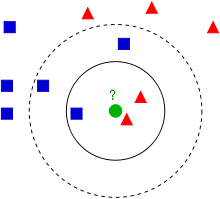
\includegraphics[height=1.5in,width=1.6in]{./images/KNN.png}
    \caption{\knn }
\end{figure}
% WHY USE KNN
Arguments supporting the usage of \knn are tremendously
dominant in the task of digit recognition. The first and most significant
reason lies in the the simplicity of its implementation. Another dominant factor is 
that the \knn  has decent performance (prediction accuracy) if given sufficent
amount of training data. Hence, we cannot reject the temptation of using \knn
as a baseline classifier.

% PROBLEM OF KNN AND SOLUTION
However, the weakness of \knn lies in its vulnerability to badly scaled
dimension when the distance between arbitrary data objects is computed. This
is especially true when the input data has extremely large number of features.
To solve this problem, we apply min-max normalization after the preprocessing
step. Another issue we concerned about is the determination of the range of
voting. In other word, how many neighbours are allowed to participate in the
decision process of one object's class membership? As stated previously, we
apply the classic technique Cross Validation to determine the parameter $k$ so
as to reach the optimal performance.

\subsection{Neural Network}
% INTRODUCTION TO NEURAL NETWORK
In the field of machine learning, {\bf neural networks} are computational models
inspired by animals' central nervous systems (in particular the brain) that
are capable of machine learning and pattern recognition. They are usually
presented as systems of interconnected "neurons" that can compute values from
inputs by feeding information through the network. Another name for neural
network is artificial neural network (ANN).

% GRAPHICAL REPRESENTATION
The graphical representation of variables are as follows. The nodes in input
layer represents the input features of each training entity. Those nodes in
hidden layer corresponds to the learned features, served for final regression
or classification decision of that entity. And the only node in output layer
corresponds to the regression or prediction decision.

\def\layersep{2.5cm}
\begin{figure}[h]
\begin{center}
\begin{tikzpicture}[shorten >=1pt,->,draw=black!50, node distance=\layersep]
    \tikzstyle{every pin edge}=[<-,shorten <=1pt]
    \tikzstyle{neuron}=[circle,fill=black!25,minimum size=17pt,inner sep=0pt]
    \tikzstyle{input neuron}=[neuron, fill=green!50];
    \tikzstyle{output neuron}=[neuron, fill=red!50];
    \tikzstyle{hidden neuron}=[neuron, fill=blue!50];
    \tikzstyle{annot} = [text width=4em, text centered]

    % Draw the input layer nodes
    \foreach \name / \y in {1,...,4}
    % This is the same as writing \foreach \name / \y in {1/1,2/2,3/3,4/4}
        \node[input neuron, pin=left:Input \#\y] (I-\name) at (0,-\y) {};

    % Draw the hidden layer nodes
    \foreach \name / \y in {1,...,5}
        \path[yshift=0.5cm]
            node[hidden neuron] (H-\name) at (\layersep,-\y cm) {};

    % Draw the output layer node
    \node[output neuron,pin={[pin edge={->}]right:Output}, right of=H-3] (O) {};

    % Connect every node in the input layer with every node in the
    % hidden layer.
    \foreach \source in {1,...,4}
        \foreach \dest in {1,...,5}
            \path (I-\source) edge (H-\dest);

    % Connect every node in the hidden layer with the output layer
    \foreach \source in {1,...,5}
        \path (H-\source) edge (O);

    % Annotate the layers
    \node[annot,above of=H-1, node distance=1cm] (hl) {Hidden layer};
    \node[annot,left of=hl] {Input layer};
    \node[annot,right of=hl] {Output layer};
\end{tikzpicture}
\end{center}
\caption{Neural Network Diagram}
\end{figure}

An ANN is typically defined by three types of parameters: (a) The
interconnection pattern between the different layers of neurons (b) The learning
process for updating the weights of the interconnections (c) The activation
function that converts a neuron's weighted input to its output activation.

Mathematically, a series of training entities are provided. We just take one
entity $\mathbf{x}$ as example. The entire input layer are fed by the instance
$\mathbf{x} = (x_1, ..., x_n)$. And the information passed in to the $j$-th
hidden nodes $a_j$ is computed by 

\begin{align}
    a_j = \sum_{i} w_{ji} x_i 
\end{align}

For each hidden node, after receiving the information from input layer,
derive its activated value $y_j$ through what it acquire by activation function $h(x)$:

\begin{align}
   y_j = h(a_j) = h(\sum_{i} w_{ji} x_i)    
\end{align}

Since we formulate digit recognition as a multi-class classification problem,
the activation function in the output layer should be a generalized logistic
function, that is, softmax function. Here, we provide the definition of
softmax function as follows: given a set of 

\begin{align}
    \sigma({\bf z}) = \frac{e^{{\bf z}_j}}{\sum_{k=1}^{K} e^{{\bf z}_k}}
\end{align}

Note that the input vector $\mathbf{z}$ should be offset down by maximum
element of that vector, in which way the "blowup" of every individual
exponential term can be avoided. This is actually a common problem in the
scientific computing.

To train neural network model, we need to feed the neural network with a
series of entities. The flow of information, while doing training,
involves in two stages: forward propagation and backward propagation.  In the
stage of forward propagation, the network accept a new training entity at input layer
, pass the value forward until output layer and finally evaluate the
prediction over that particular entity. Since the error (difference
between prediction label and groudtruth label) was derived, it comes to the
stage of the back propagation. In this stage, the pre-computed error was
passed back towards the input layer so as to update the parameters (weight
matrix). We can keep on feeding training entity to this neural network until
convergence.

% BACKPROPAGATION
The stage of backward propagation is much more complicated. On the output
layer, the error is simply as the difference of output and activated value on
that unit. However, the error of hidden nodes are computed similar to the
propagation in the first forward stage. Formally, the error $\delta_j$ of node indexed by
$j$ in previous layer can be represented as 

\begin{align}
    \delta_i = h'(a_j) \sum_{k} w_{kj} \delta_k
\end{align}

Every nodes on one hidden layer first collects all
error from next layer, summarize them as its error made by itself and finally
update the weight matrix. Note that there is no error for neurons on input
layer. 

\begin{figure}[h]
    \centering
    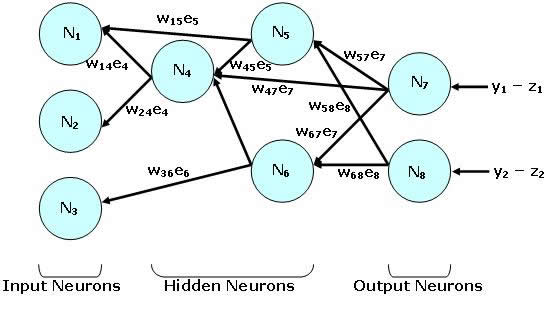
\includegraphics[height=2.2in,width=3.8in]{./images/BackPropagation.jpg}
    \caption{Backward propagation of Neural Network}
\end{figure}


% WHY USE Neural Network
As to the motivation of using neural network, one most significant factor
comes to the fact that Neural Networks are usually employed as one universal
function approximator. Formally, if given sufficent hidden nodes, the neural
network model can approximate any function to arbitrary precision. Ituitively,
we can treat the digit number as a function of a series features. In original
setting, these features are gray value of every pixel. If preprocessed by PCA,
the features become the principal components chosen by us. 

% IMPLEMENTATION DETAIL
There are also several concerns for the implementation of Neural Network model.
The first one coming to our mind is the number of hidden nodes for usage. We
turned to various experiment report for the parameter optimization of neural
network on digit recognition. It turns out that about five to six layers of
nodes will result in astonishingly good performance. One convincing approach
to address this problem is to cross validate on the network structure, but
this requires a large computational cost.
Another concern is the determination of leraning rate $\alpha$. The third one
is selection of activation function for hidden nodes. Typically, there are a
few options: $tan(x)$, $log(x)$, $exp(x)$. We can cross validate over all
these activation function for nodes of each layer. Last but not in the least,
 how to avoid overfitting remained a challenging issue. Theoretically, early
 stopping and fine-tune regularization parameters are both suitable approaches
 to avoid overfitting of neural network. However, our attempted implementation
 does not incorporate any of them. 

\subsection{Deformation Model}

\section{Result} \label{Comparison}

\subsection{Commitment History}
{\bf Progress \#1 issued at March 29 }

1. Jimmy Lin: We work out initial version of **Principle Component Analysis**(PCA), and
submit it with KNN classification model. In this submission, we acquire an
prediction accuracy of **0.96886** and ranked at **148** at that date. 

2. Jimmy Lin: We also tried Random Forest method based on PCA 100 pricipal components and
achieve **0.95457** accuracy.

{\bf Progress \#2 issued at April 14 }

1. Jimmy Lin: C-SVM with preprocessed data by **Principle Component Analysis** (100
principal components). The prediction accuracy achieved is **0.91043**.

2. Jimmy Lin: NU-SVM with the same configuration achieves accuracy **0.89743**.

3. Jimmy Lin: code up our own implementation of neural network. However,
our implementation does not come out with satisfyingresult, perhaps because of
no mechanism to avoid overfitting.  

{\bf Progress \#3 issued at April 16 }

1. Jimmy Lin: Reference to libsvm's C-SVM method with normalization preprocessing achieves **0.93571**.

2. Jimmy Lin: Implement Majority Voting Ensemble Method, containing PCA-KNN, KNN, libsvm-All-CSVM,
achieves **0.96714**. Still no breakthrough.

{\bf Progress \#4 issued at April 24 }

1. Jason Yang: Apply Cross Validation Techniques to determine the optimal parameters of
PCA-KNN model. The prediction accuracy achieved is **0.97300** and in the
meanwhile, we refresh our ranking to 99.


{\bf Progress \#5 issued at April 26 }

1. Jason Yang: Turn to the implementation of neural network implementation in
Deep Learning Toolbox. And achieves an accuracy of ** **.

{\bf Progress \#6 issued at April 27 }

1. Jimmy Lin: read the paper of deformation model and code up for it. To
compute the solution by this model, we make use of over 50 UTCS Linux machine
to run in parallel. However, our implementation only achieves **0.92629**,
which does not reach our expectation.

\subsection{Ranking on Kaggle Competition}

Our optimal solution model {\bf PCA-KNN} ranks at 99 of the leader board.
Following is the snapshot of our position on that leaderboard.

\begin{figure}[h]
    \centering
    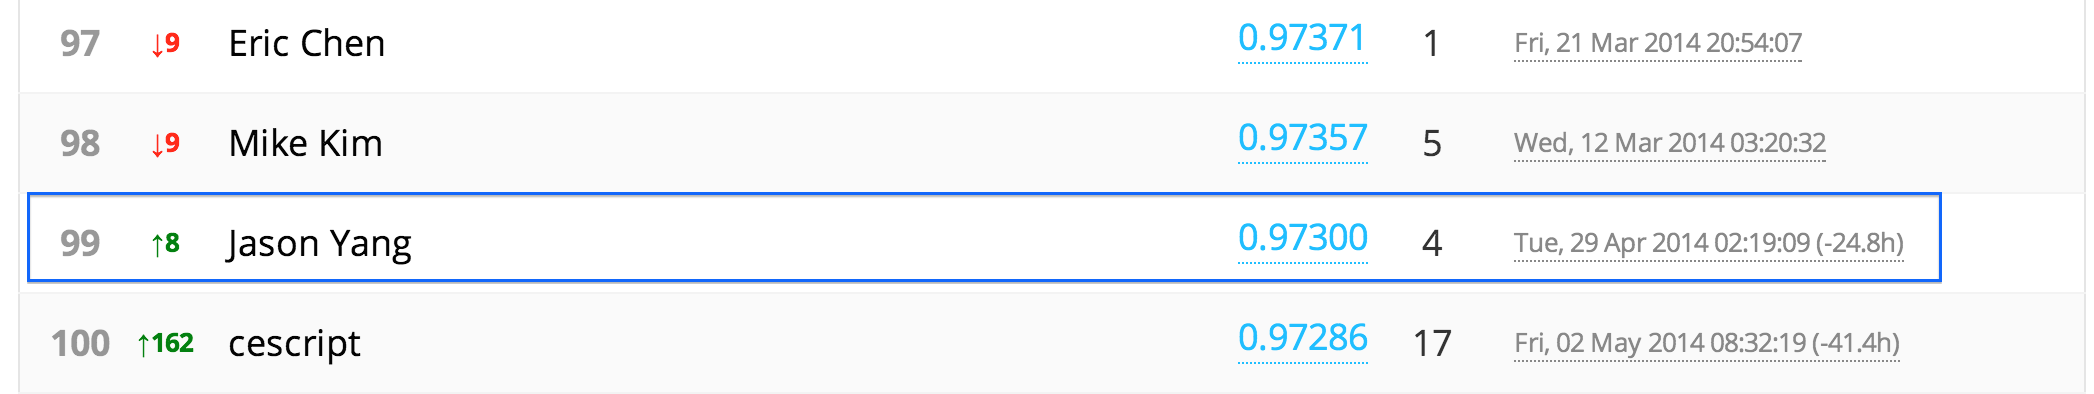
\includegraphics[width=5.5in,height=1.2in]{./images/Rank.png} \\
    \caption{Ranking of our best solution (PCA-KNN model)}
\end{figure}

\begin{figure}[h]
    \centering
    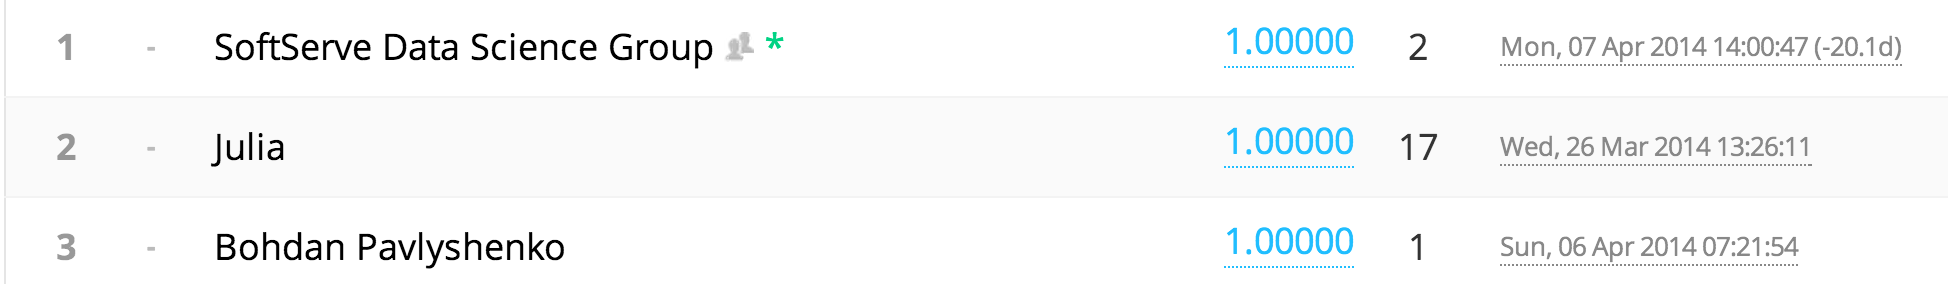
\includegraphics[width=5.5in,height=0.9in]{./images/topRank.png} \\
    \caption{Performance of top solution in this competition}
\end{figure}
For further details about this leader board, please visit
\begin{center}
\url{http://www.kaggle.com/c/digit-recognizer/leaderboard} 
\end{center}

\subsection{More about Optimal Solution: PCA-KNN}
\section{Conclusion and Discussion} \label{Conclu}

% TODO: some summarization
High model complexity does not indicate high performance. It is true that the academia
has developed plenty of theoretically elegant model, most of which are
difficult to implement and understand. However, they are not necessarily suitable
for any problem on any circumstance. In our experiment, the PCA-KNN model is
simplest in both theoretical and practical respects, but it achieves highest
performance for (maybe particularly) this digit recognition problem.

Sometimes, the quality and quantity of the dataset matters a lot. It has been
a long debate over whether the dataset plays more significant role over the
model in the area of data mining and machine learning or whether model is
supposed to be more important. It can be extremely hard to say one is always
over the other. Nevertheless, from our project, we can say that sometimes the
quantity really does matter, and even take a dominant role. The observation
supporting this argument is that the \knn model does not perform well when the
given training data is of small size, comparing to the case of large size
input like 42,000 training images.  


% TODO: further improvement
When it comes to the possible further improvement, the first come to our mind
is to attempt to make full use of the neural network architecture. Just as
stated in the implementation details of neural network, we can actually cross
validate on various parameters, including the network structure, activation
function for each layer, and the regularization parameter (or iteration number
if early stopping technique is used). It is true that the searching space
would be rather large if we consider to optimize over such many factors. The
way to practically touch the limit of neural network model in digit
recognition problem is to make use of our existing distributed computing
framework.

\section{References}


\small{
% FEATURE EXTRACTION
[1] Liu, C. L., Nakashima, K., Sako, H., \& Fujisawa, H. (2003). Handwritten
digit recognition: benchmarking of state-of-the-art techniques. {\it Pattern
    Recognition}, {\bf 36(10)}, 2271-2285.

% NEURAL NETWORK
[2] Le Cun, B. B., Denker, J. S., Henderson, D., Howard, R. E., Hubbard, W., \&
Jackel, L. D. (1990). Handwritten digit recognition with a back-propagation
network. In {\it Advances in neural information processing systems.}

% NEURAL NETWORK
[3] LeCun, Y., Jackel, L. D., Bottou, L., Brunot, A., Cortes, C., Denker, J.
S., \& Vapnik, V. (1995, October). Comparison of learning algorithms for
handwritten digit recognition. In {\it International conference on artificial
    neural networks} {\bf (Vol. 60)}.

% THEORY: DEEP LEARNING PAPER
[4] Hinton, G. E., Osindero, S., \& Teh, Y. W. (2006). A fast learning
algorithm for deep belief nets. {\it Neural computation}, {\bf 18(7)}, 1527-1554.

% APPLICATION: DEEP LEARNING ON DIGIT RECOGNITION
[5] Ciresan, D. C., Meier, U., Gambardella, L. M., \& Schmidhuber, J. (2010).
Deep, big, simple neural nets for handwritten digit recognition. {\it Neural
    computation}, {\it 22(12)}, 3207-3220.

% Deformation method
[6] Keysers, Daniel, et al. "Deformation models for image recognition."
{\it Pattern Analysis and Machine Intelligence, IEEE Transactions} on 29.8 (2007):
1422-1435.
}

\newpage
\appendix
%% code reference setting
\definecolor{keywords}{RGB}{0,0,0}
\definecolor{comments}{RGB}{0,0,0}
\definecolor{red}{RGB}{0,0,0}
\definecolor{green}{RGB}{0,0,0}
\lstset{language=Python, 
        basicstyle=\ttfamily\small, 
        keywordstyle=\color{keywords},
        commentstyle=\color{comments},
        stringstyle=\color{red},
        showstringspaces=false,
        identifierstyle=\color{green},
        procnamekeys={def,class}}

\section{Matlab Implementation of PCA-KNN Classifier}
\subsection{Driver Script}
\lstinputlisting[language=Matlab]{../codebase/PCA-KNN/src.m}
\subsection{PCA-KNN Routine}
\lstinputlisting[language=Matlab]{../codebase/PCA-KNN/estimate_labels.m}
\subsection{Cross Validation}
\lstinputlisting[language=Matlab]{../codebase/PCA-KNN/crossval.m}
\newpage

\section{Our Attempted Implementation of Neural Network}
\lstinputlisting[language=Matlab]{../codebase/NN.m}
\newpage


\section{Matlab Implementation of Deformation Model}
\subsection{IDM Classifier}
\lstinputlisting[language=Matlab]{../codebase/IDM_Deform.m}
\newpage
\subsection{Distributed Computation}
\lstinputlisting[language=Python]{../codebase/IDM/getListOfAvailableHosts.py}
\newpage

\section{Matlab Implementation of Ensemble Method}
\subsection{Ensemble Method by Majority Voting}
\lstinputlisting[language=Matlab]{../codebase/Ensemble.m}

\newpage
\section{Invocation of other libraries}
\subsection{Deep learning Toolbox}
\lstinputlisting[language=Matlab]{../codebase/DPNN.m}
\subsection{Libsvm}
\lstinputlisting[language=Matlab]{../codebase/NU_SVM.m}

\end{document}
